% !TEX TS-program = LuaLaTeX

\DocumentMetadata{}
\documentclass[twocolumn]{willarticle}
\usepackage{geometry}
\geometry{margin=1cm}
\usepackage{listings,refstyle,framed,biblatex,hyperref}
\lstset{basicstyle=\small\ttfamily,frame=lrtb}

\newcommand\Principle[1]{\begin{framed}\bfseries Principle: #1\end{framed}}

\bibliography{acoustics}

\begin{document}

\title{What engineers should learn from software engineering: Updating the Bellhop repository with Open Science best practices}
\author{William S. P. Robertson, Chung Fang, and Anthony C. Zander}

\maketitle

\begin{abstract}\em
This article discusses best practices in open science research dissemination through the lens of documenting and modernising the `Bellhop' codebase for underwater acoustics ray-tracing.
\end{abstract}

\section{Introduction}

The use of open science practices has been increasing since the discussion of reproducible research in the 2000s, alongside a shift towards open access publication and the growing popularity of open data repositories.
There is now critical mass in the technologies used for the dissemination of open science research that further prescriptive guidance on appropriate practices can now be given.
This article uses the `Bellhop' underwater acoustics codebase as a case study to document and illustrate these practices.

Reproducible research and open science are critical for researchers to continue to `stand on the shoulders' of their predecessors in the advancement of science.
Every time a typo in an equation in a published paper is dutifully copied into a script as another researcher tries to build on what they have done, there is risk of wild goose chases, significant confusion as results are not as intended, and leads to wasted time and effort.
I personally have published equations with typos in them, and I've tried to reproduce others' work from equations that were plain incorrect in their typeset published form.
I've also looked in awe at papers published which only describe what must be monumental amounts of code, that I could not even dream of reproducing in the time allotted for a project -- let alone extending the techniques.
There are now better ways.

We should now be encouraging all active researchers to publish not just a description of their methods alongside their results, but to also publish in parallel their code.
In particularly, we should be encouraging PhD students to do so --- those who are well placed to learn good habits.
Intellectual property can of course be a concern in some disciplines or projects, and we should contain to hold tight what is truly valuable IP.
On the other hand, in most cases if we are willing to publish our papers we should also be willing to publish our code.

Publishing code can be as simple as uploading the raw scripts and libraries that were used to create the results of a paper.
If you are anything like me, you will often come back to the same pieces of code over time, and providing general interfaces and options often quickly follows.
The scientific community has seen some extraordinary open source contributions over the decades, many of which provided so much utility to so many researchers that it is hard to imagine how far we would have been set back if those software packages were never released openly.

Bellhop is an example of a long-standing open source software package that has enabled a large body of additional research to be built upon the foundation it provides.
It makes for an interesting case study to discuss open science, as it is currently published openly, and widely used by the research community, with an ecosystem of tools that have been built to interface with it.
Nonetheless, it is a `legacy' codebase in the sense that it is reliable and stable, and as a result does not make use of modern software development practices.
This work does not seek to improve the science that Bellhop provides, merely to enhance the packaging of this work to hopefully enable more people to use and learn from it.

The following key additions were undertaken to modernise the Bellhop codebase:
\begin{itemize}
\item Modern build system for better portability and accessibility
\item Automatic code documentation, including dependency graphs
\item Regression and unit testing suite
\item Code coverage reporting of the test suite
\item Coding standards (`linter')
\item Easy build systems
\item Online repository hosting
\end{itemize}
Building engineering software using these features helps mitigate the risk of unknown errors in the code, promotes reproducibility, and largely comes `for free' using modern programming tools and libraries.

\section{Bellhop's context}

Bellhop is an open source Fortran program for calculating underwater acoustic phenomena using ray tracing algorithms \parencite{porter2025-foa}.
It is written and maintained by Michael B. Porter, with early development in the 1980s (first release 1983 with Homer Bucker, Naval Ocean Systems Center), and continuous and active development through the 2000s and 2010s \parencite{porter2024-at}.
Wrappers for Bellhop have been provided in both the modern packages for Python \parencite{chitre2025-arlpy} and Julia \parencite{chitre2025-jl}, and in fact the original Bellhop codebase includes both a wrapper and a translation of the code into Matlab.
In the 2020s, another research group translated the codebase to C++ and CUDA in order to take advantage of multi-processor and GPU architectures \parencite{jaffe2025-bellhopcuda}.
Others have experimented with graphical user interfaces for Bellhop \parencite{duncan2025-actup}, which can be very useful from a pedagogy and ease-of-use perspective.

With more modern implementations and wrappers, we might question whether the Fortran source code is still of relevance.
As the Bellhop authors provide both Fortran and Matlab implementations, we can make a direct performance comparison: the Fortran code runs approximately an order of magnitude faster than the Matlab code, which makes for an easy argument that the low-level Fortran (or C++) codebases should be retained.
However, the legacy executables for Bellhop use an unstructured plain text approach to setting up simulation parameters.
This approach was typical for programs written in an era before structured text languages such as JSON, YAML, or TOML, and before `keyval' interfaces in general, were commonplace.
In the days of well-structured, readable, and easily parsable input files, the Bellhop user interface can be seen as somewhat cryptic and error-prone, particularly on account of the large number of options it now allows for.
Providing a more useful interface for controlling Bellhop's many input parameters is a significant part of modernising the codebase.

\section{Open science additions to Bellhop}

This section outlines the main changes to the Bellcode codebase that we have undertaken.

\subsection{Modern build system}

Bellhop uses the venerable Make system for building the source files into executables. Despite its age, Make is an excellent cross-platform and technology-agnostic tool for managing code.
For Bellhop, little was needed to successfully execute \verb|make|, resulting in \verb|bellhop.exe| and \verb|bellhop3d.exe| being available to install and use.

However, Make is not always easy to configure in ways that promote reproducibility and portability.
For instance, Bellhop's use of Make relied on the user to edit the Makefile directly to insert or edit the necessary compile flags for their operating system and computer platform.
If your system did not match the system used by the last person that uploaded the package code, you would need to debug and fix the configuration using trial and error, a search engine, or perhaps an AI assistant (!).
In our case, only small changes were needed (see \Figref{makefile}) to allow the Bellhop Makefile to automatically detect the platform (not heavily tested), and enable/disable certain flags depending on other contexts.

\Principle{Users should be able to build your code without needing to configure it.}

Despite the success of the Make build system, it is not set up to manage modern package building environments which need to manage dependencies, encapsulation, and so on.
For our Bellhop repository, the Hatch build system has been adopted for running the test suite, building documentation 

\begin{figure*}
\begin{lstlisting}
# Detect architecture
UNAME_M := $(shell uname -m)

# Base flags (common to all)
FFLAGS_BASE = -g -Waliasing -Wampersand -Wsurprising -Wintrinsics-std \
                 -Wno-tabs -Wintrinsic-shadow -Wline-truncation \
                 -std=gnu -frecursive

# Optimisation flags (common, but not used for coverage)
FFLAGS_OPTIM = -O2 -ffast-math -funroll-all-loops -fomit-frame-pointer

# Coverage flags (for GCOV code coverage analysis)
FFLAGS_COVERAGE = -fprofile-arcs -ftest-coverage -fcheck=all

# Arch-specific flags
ifeq ($(UNAME_M),x86_64) # Windows/Intel/Linux Intel
    FFLAGS_ARCH = -march=native -mtune=native
else ifeq ($(UNAME_M),arm64) # Apple Silicon
    FFLAGS_ARCH = -mcpu=apple-m2
else ifeq ($(UNAME_M),aarch64) # Linux ARM (e.g., Raspberry Pi, ARM server)
    FFLAGS_ARCH = -march=armv8.5-a
else
    $(warning Unknown architecture $(UNAME_M), using generic flags)
    FFLAGS_ARCH =
endif
\end{lstlisting}
\caption{Snippet from the Bellhop Makefile to automatically detect the platform for selecting compiler flags.}
\label{fig:makefile}
\end{figure*}

\subsection{Automatic code documentation}

There are several widely-used automatic code documentation tools, including Doxygen and Sphinx.
Because Bellhop is written in Fortran, the FORD tool was selected to generate its base documentation.
Because it is tightly coupled to Fortran conventions, FORD required basically no setup or configuration to `just work'.
Only minor changes to the Bellhop Fortran sources were needed for the comments in the file to match FORD's expectations.
A modified comment prefix (\verb|!!|) creates specially tagged documentation strings that are extracted for the summary online documentation (\Figref{ford-modules}), which presents an overview of the collections of files, modules, procedures, and so on, in the codebase.

\Principle{A system for automatic code documentation promotes consistency and good code style; it encourages explicit documentation of available options and input/output specifications.}

FORD analyses the code and creates connected graphs (\Figref{graphvis}) to link files to files, modules to modules, and so on. Most importantly, this showed which source files were not being used in the Bellhop codebase, as it is provided alongside additional underwater acoustics programs — Kraken, etc.\ — with a shared library.
(If we were to repeat this process for these additional programs, it is likely that we would simply duplicate the shared source files across repositories. Generally speaking, monolithic repositories can be harder to manage as most users will only have need for a subset of the components.)

The Python interface to bellhop is documented using Sphinx (following arlpy). The Sphinx output is combined with the main FORD output to create the documentation pages.

\begin{figure*}
\centerline{\fbox{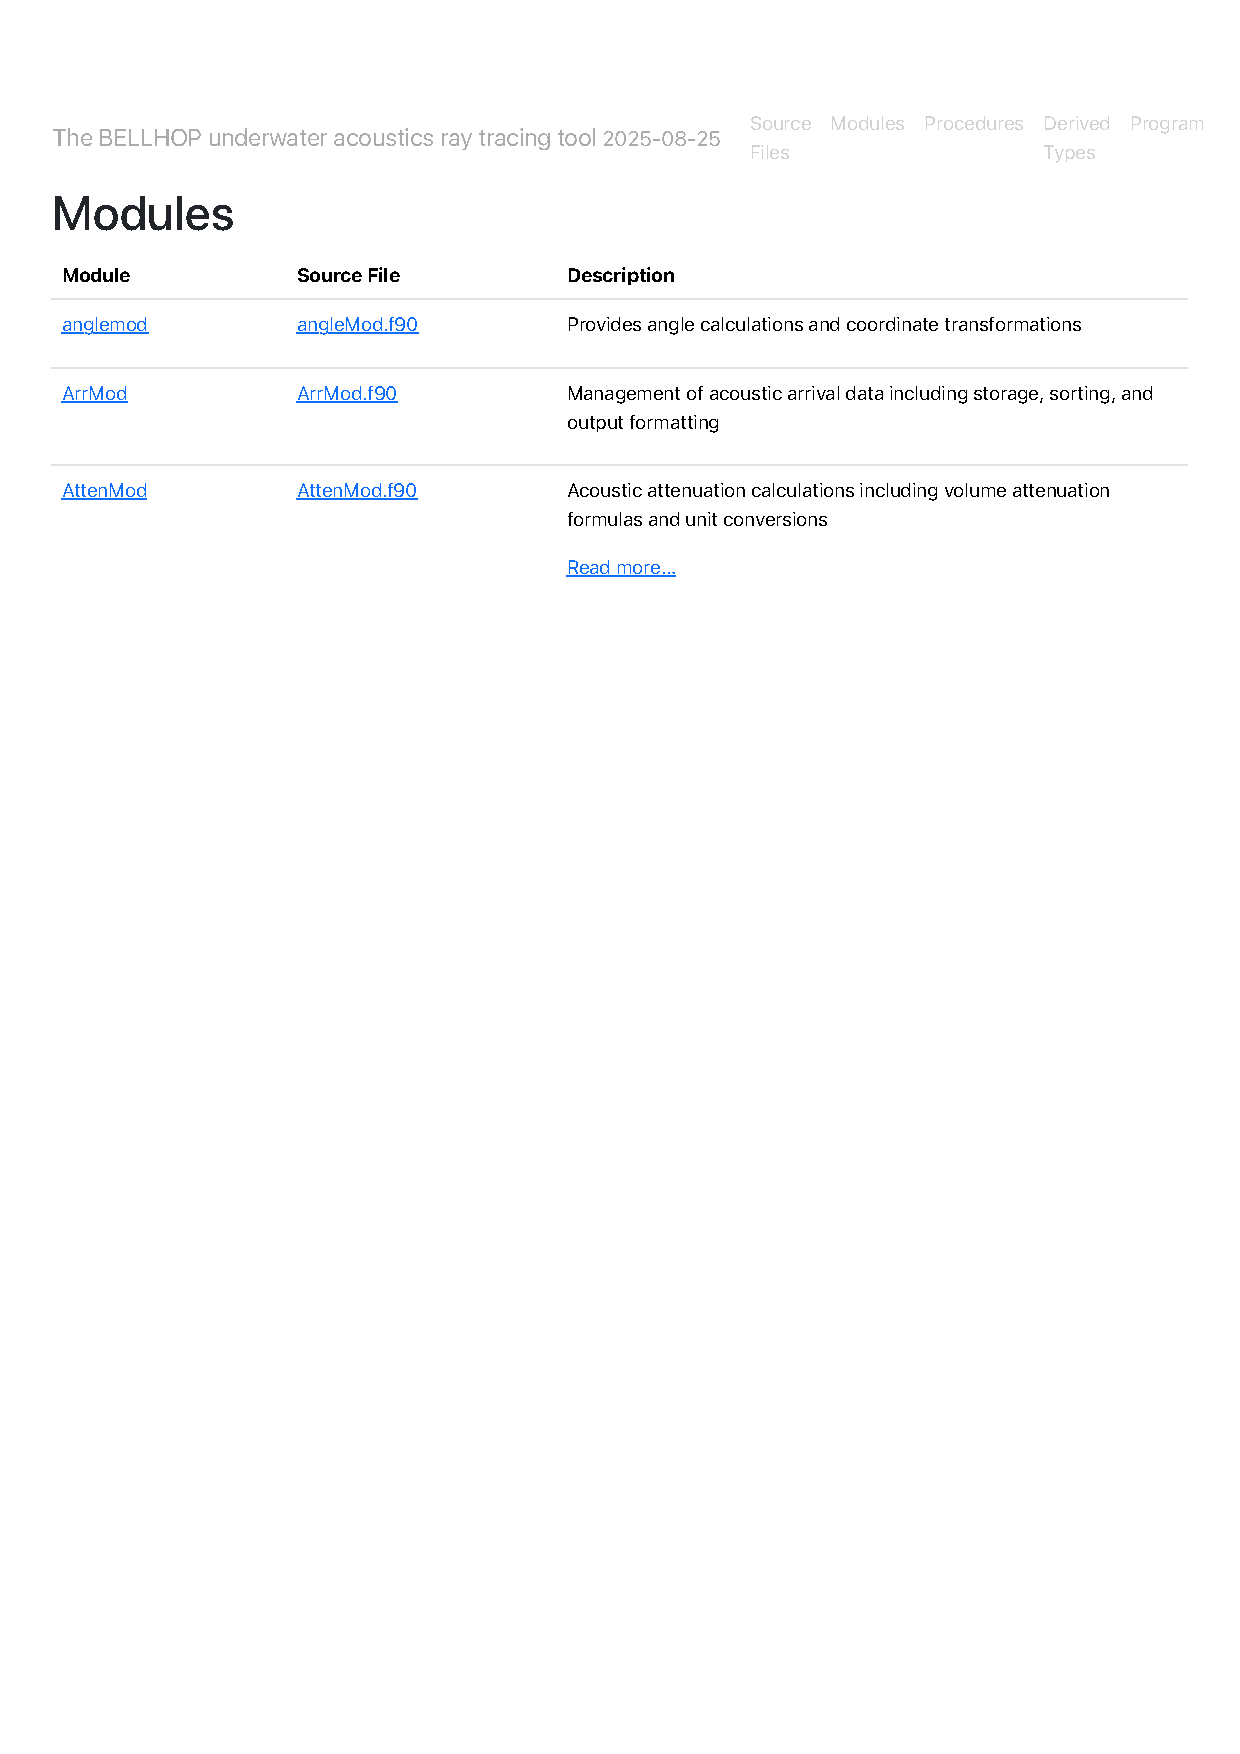
\includegraphics[width=0.8\linewidth]{fig/ford-modules-snap}}}
\caption{Example output of the FORD Modules documentation.}
\figlabel{ford-modules}
\end{figure*}

\begin{figure*}
\centerline{\fbox{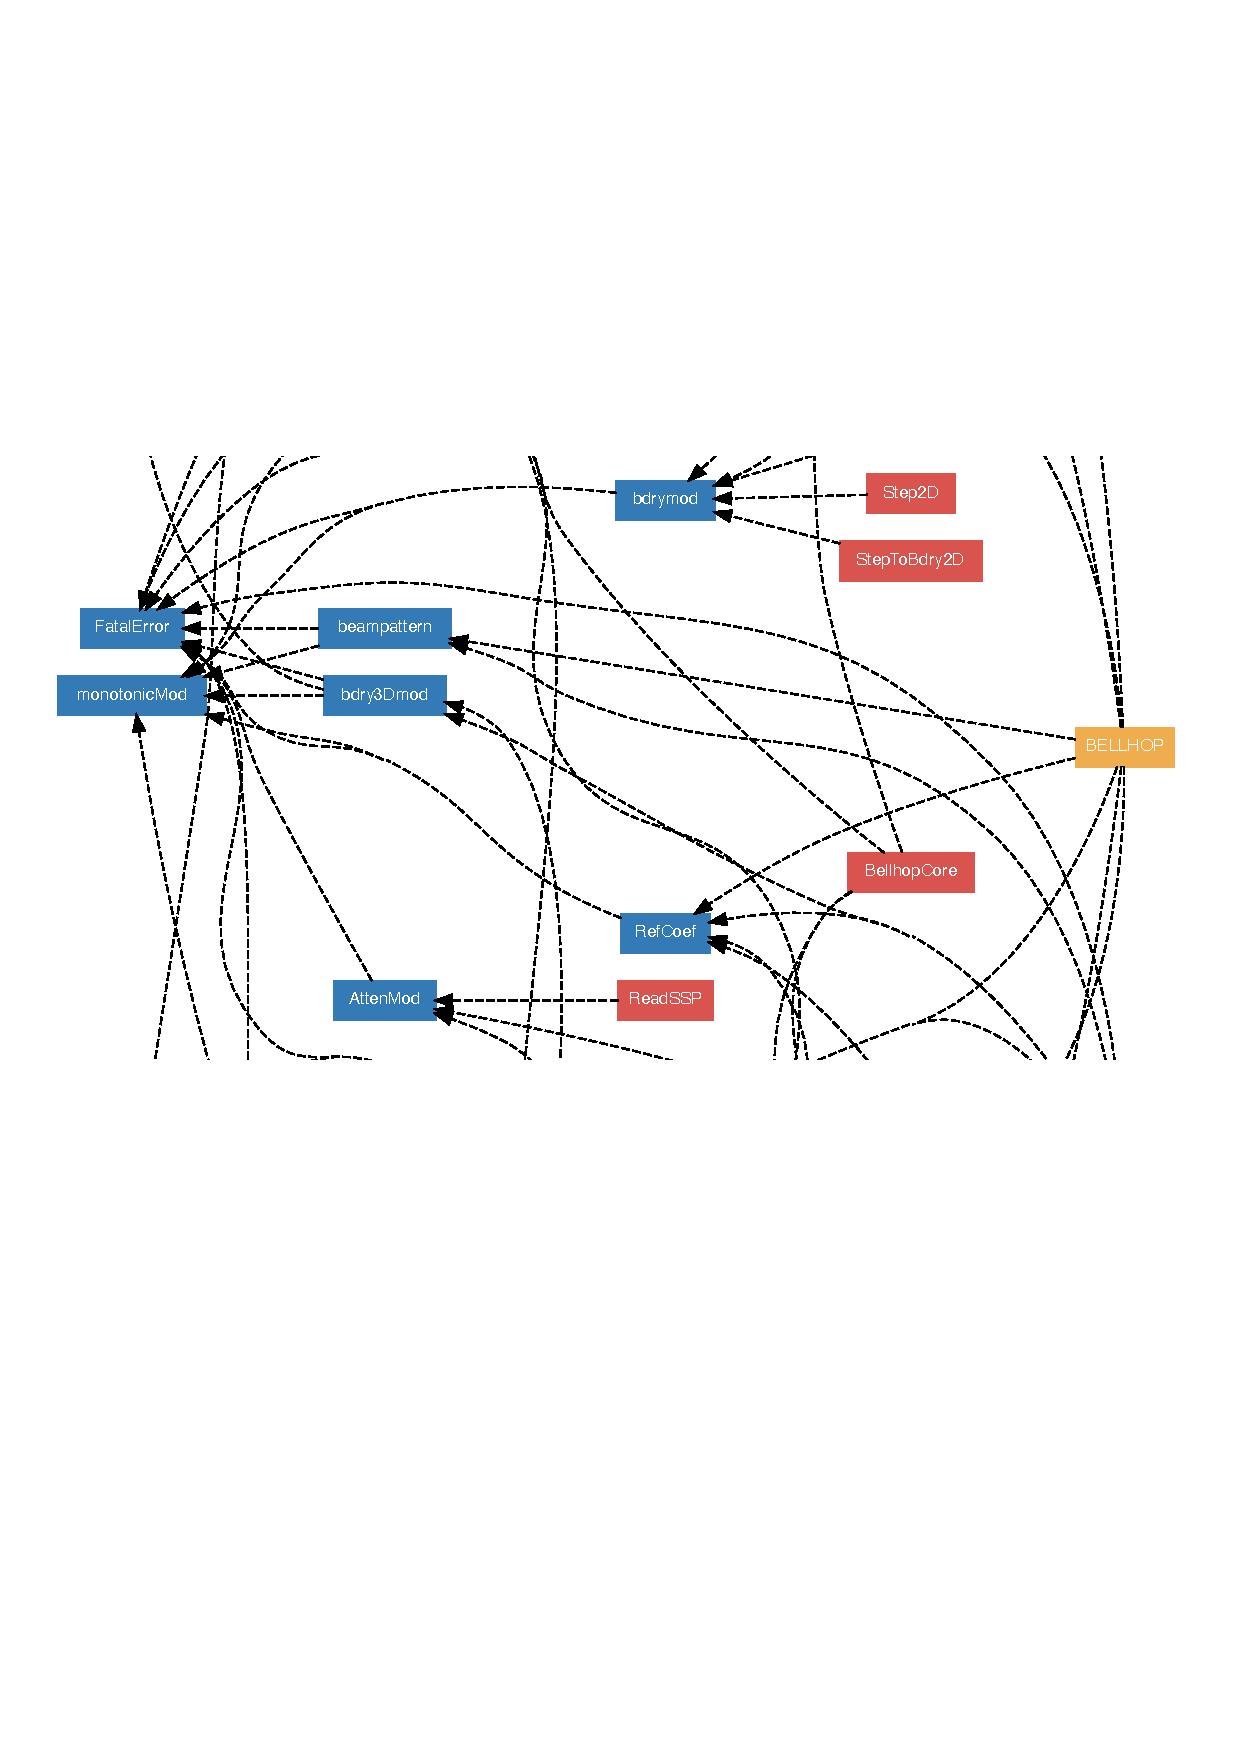
\includegraphics[width=0.8\linewidth]{fig/graphvis}}}
\caption{Extract from part of the Graphvis output from the FORD Modules documentation.}
\figlabel{graphvis}

\end{figure*}

\subsection{Regression and unit testing suite}

This is the most important element of reproducible research.
A suite of testing procedures is the cornerstone of validating that a software package produces correct output under a comprehensive range of input conditions, and that changes to the code over time do not introduce changes to the output.

\Principle{Tests should be comprehensive and written in parallel with the code itself.}

Engineering software is uniquely well-suited to many types of testing approaches, as numerical outputs can be explicitly queried.

For Bellhop, the Acoustics Toolbox distribution contains a very large number of examples, which allows verification testing that any changes to the source files do not result in execution failures.
However, these examples do not attempt to perform validity checks that their numerical output is correct.
Introducing a Python-based testing procedure was critical in being able to make changes to the Fortran sources with confidence. 

\subsection{Code coverage reporting of the test suite}

Even with good intentions to write tests as the code is written, it is difficult to manually assess whether a test suite actually checks all possible code paths of a program.
Without feedback about what is being tested, we cannot independently verify that we have enough tests.
`Code coverage' reporting is an automated approach to identifying how much of the source code is being executed when the test suite runs (\Figref{coverage}).
A source file with less than 100\% coverage is likely to have branches which are not being tested; for instance, this often occurs when a feature is provided with a range of options, and not each option is explicitly tested (\Figref{cov-detailed}). 

Code coverage is managed using the \verb|gcov| compiler tool with a separate set of build instructions through the Makefile.
As code coverage reporting literally changes the executable that is compiled, there are small numerical differences in the outputs.
Therefore, when the test suite is run in code coverage mode, the level of checking is reduced.
The reason for these differences is that finite-precision arithmetic does not operate with the same rules as for abstract mathematics.
For instance, when dealing with very small floating point numbers, it cannot be assumed that
\[
  a + (b + c) \mathop{=}\limits^{?} (a + b) + c \,.
\]
As compiler optimisation can re-arrange the order of operations, a seemingly innocuous change to the compiler rules can yield differences in output.
In fact, we also see similar behaviour when compiling the test suite on one platform versus another.

\begin{figure*}
\centerline{\fbox{
\includegraphics[width=0.8\linewidth]{fig/coverage.pdf}}}
\caption{Example of coverage report summary output. Each file contains a detailed report that shows the number of times each line of code is executed by running the test suite.}
\figlabel{coverage}
\end{figure*}

\begin{figure*}
\centerline{\fbox{
\includegraphics[width=0.8\linewidth]{fig/cov-detailed}}}
\caption{Example of coverage report detailed output. The red highlight shows code which is not run as part of the test suite.}
\figlabel{cov-detailed}
\end{figure*}

\subsection{Coding standards}

Modern `linter' tools such as \verb|ruff| (for Python) and \verb|fortitude| (for Fortran) are designed to enforce coding standards.
Code written to standard are less likely to contain subtle bugs, and minimise friction moving between codebases.
E.g., developers experience friction when there are inconsistencies with something trivial like spaces, or not, around maths operators.
When coded to standards, a new contributor does not face having to adapt to another developer's personal style.

When first used on the Bellhop repository, \verb|fortitude| reported 1168 `errors'.
These include trivial issues such as trailing whitespace in source code, long lines of code, deprecated operators, hard-coded numeric values, and so on.
To be clear, these 1168 so-called errors are not indicating there are any problems with the Bellhop code, nor that its developers were taking shortcuts in the development.
Modern linter tools by default are strict about upholding what are now considered to be best practice guidelines, but which may not have been (or could not have been) rigorously followed in years past.

Dynamic programming languages like Python often do not require variables to be `typed', unlike compiled languages such as Fortran or C in which each variable is initialised as an integer, floating point number, string, and so on.
However, static checking of code checks code structure to ensure that variables are being used in internally consistent contexts, and this type of checking can catch subtle bugs that can yield confusing errors.
To enable static checking, Python (among other dynamic languages) provides syntax to `hint' what the types of the variables and function arguments expect.
Although not used in the execution of the program, the consistent use of these type hints provides a number of benefits and is now considered best practice.
At time of writing, the \verb|mypy| type checking program is most commonly used for production Python code.
When first executed on the Bellhop python code (after substantial development from its ARLpy base), a total of 337 errors were reported.

\Principle{Use lint and type checking tools to ensure that code is written using best-practice guidelines.}

For legacy code, it may not be feasible (or sensible) to fix all of these identified issues.
Several 

\subsection{Easy build systems}

These powerful development tools are all well and good, but need to be easy to run without remembering particular configuration options or setup steps.

\Principle{Use standard build tools and set them up to minimise friction by automating common steps.}

Traditional workflows used \verb|make|, and modern Python tools such as \verb|hatch| and |\verb|uv| provide more complex environment setup options.
The Bellhop repository is set up with Hatch used for running the main development tools, with a transparent user interface provided by Make to help streamline shifting from one build process to another (e.g., from Hatch to UV), in the future.

The Make interface is as simple as (\verb|make help|):
\begin{verbatim}
  CODE BUILDING
    [all] - default — build binaries
    clean - remove all temporary files
  install - copy binaries into ./bin

  CODE CHECKING
     test - run test suite
cleantest - rebuild entire codebase
            and then run test suite
     lint - run code linters
      doc - build online documentation
      cov - run code coverage process

  DEVELOPMENT TOOLS
     push - push code changes to repo
            (checks lint, test first)
\end{verbatim}

\subsection{Online repository hosting}

This project is hosted on Github, likely the most popular online repositories at time of writing.
Github provides generous support educational and open source users.
A publicly hosted project provides a stable home to access the work, but online platforms offer many desirable features, including collaboration and project management tools (such as pull requests and issue tracking), ability to serve websites based on project documentation, and so-called `continuous integration' workflows.

\Principle{Researchers should aim to publish their code through online repositories, which most easily allow for dissemination and collaboration of their work.}

Very recently (at time of writing), it is now possible to integrate AI agents into online repositories, who can run, analyse, and suggest changes to code directly.


\paragraph{Online documentation, including examples}

\paragraph{Continuous Integration through Github Workflows}

\section{Examples}

\section{Conclusion}

\onecolumn
\clearpage
\printbibliography

\end{document}
